\documentclass[a4paper,11pt]{kth-mag}
\usepackage[T1]{fontenc}
\usepackage{textcomp}
\usepackage{lmodern}
\usepackage{amsmath}
\usepackage[swedish,english]{babel}
\usepackage{modifications}
\usepackage[usenames,dvipsnames,svgnames,table]{xcolor}
%\usepackage[toc]{glossaries}
\usepackage{pgfplots}
\usepackage{graphicx}
\usepackage{pgfplotstable}
\usepackage{afterpage}

\usepackage{rotating}

\graphicspath{ {img/} }
\pgfplotsset{width=12cm,compat=1.9}

%\newglossaryentry{computer}{
%  name=computer,
%  description=
%  {is a programmable machine that receives input,
%    stores and manipulates data, and provides
%    output in a useful format}
%}
%\newglossaryentry{MLE}{
%  name=Maximum Likelihood Estimate,
%  description=
%  {\todo yolo}
%}
%\newglossaryentry{BFS}{
%  name=Breadth First Search,
%  description={Basic search algorithm where each previously unexamined connecting neighbor of a node is examined in a iteration, and the queued to be subject for the next iteration.}
%}
%\newglossaryentry{wordnet}{
%  name=WordNet,
%  description={WordNet\cite{wordnet} is a lexical database for English. WordNet has nouns, verbs, adjectives and adverbs grouped into sets of cognitive synonyms (synsets), each expressing a distinct concept. These synsets are interlinked by means of conceptual-semantic and lexical relations.}
%}
%\newglossaryentry{jaws}{
%  name=JAWS,
%  description={JAWS\cite{jaws} is a library providing API methods for accessing synset relations in \gls{wordnet}}
%}
%
%\newglossaryentry{superword}{
%  name=hypernym,
%  description={A word relation implying less specific meaning. For example, \emph{color} is a hypernym of \emph{red}.}
%}


\newcommand{\todo}{ ... }
\newcommand{\ngram}{$n$-gram}
\newcommand{\category}{restaurant category }  % may become plural
\newcommand{\numAnnotated}{1000}
\newcommand{\numClassifierAproaches}{2}

\newcommand{\ysc}{Modified Kneser-Ney classifier}

\newif\ifhasStudiedFailures
\hasStudiedFailuresfalse

\newcommand{\loremipsum}{
  {\color{lightgray}
  PLACEHOLDER: Fruit two greater fifth over every. In female fourth good wherein herb
  Waters yielding itself. Female greater. Hath in, second appear tree in.
  Him, it seasons. Upon. Good you're. Winged green. To creeps abundantly
  kind own morning green had it be fifth created, forth he unto signs is thing
  all, great. Place night Gathering upon were forth light deep. Abundantly.
  Kind air beginning his void seed it dry. Own and spirit may dry abundantly
  beast good forth. The fifth beginning. Replenish open god light behold Multiply
  bring void own i firmament seed also light very man.

  }
}

\newcommand{\gls}[1]{TODO(#1)}
%\makeglossaries

\title{Mining opinions from local business reviews:\\ A technical walk-through.}

\subtitle{Getting that degree would be nice1 before I go work full time}
\foreigntitle{This is the Swedish title}
\author{Mattis Kancans Envall}
\date{June 2016}
\blurb{Master's Thesis at CSC\\Supervisor: Johan Boye\\Examiner: Viggo Kann}
\trita{TRITA xxx yyyy-nn}


\begin{document}
\frontmatter
\pagestyle{empty}
\removepagenumbers
\maketitle
\selectlanguage{english}
\begin{abstract}
%line are becoming one of the most important resources when comparing businesses, services and products.
%for more reliable conclusions as more opinions can be taken into account, but it also poses a problem,
%ers can process.
%
%apable to handle big quantities of data, which suggests potential for using computers as aid when
%
%
%escribes on a technical level how to develop a system that
%mmaries, and prodives detailed studies of a few key concepts required
%
\end{abstract}


\clearpage
\begin{foreignabstract}{swedish}
\loremipsum

\end{foreignabstract}
\clearpage
\tableofcontents*

%\glsaddall
%\printglossaries

\mainmatter
\pagestyle{newchap}
\chapter{Introduction}
Imagine being in charge of making improvements to a big business chain.
How would you know what changes to make? Customer feedback could certainly
help inform decisions; but traditional methods of gathering such feedback,
such as surveys or interviews, require planning and resources.
With todays extensive internet usage, it is likely that the answers you need already
are available online, however, for big business chains there could easily be tens of thousands of reviews ---
far more than a human reader can reasonably process.
Thus there is incentive to use computers as aid to organize,
and visualize
large quantities of opinions.

\begin{figure}[t]
  \centering
  \fbox{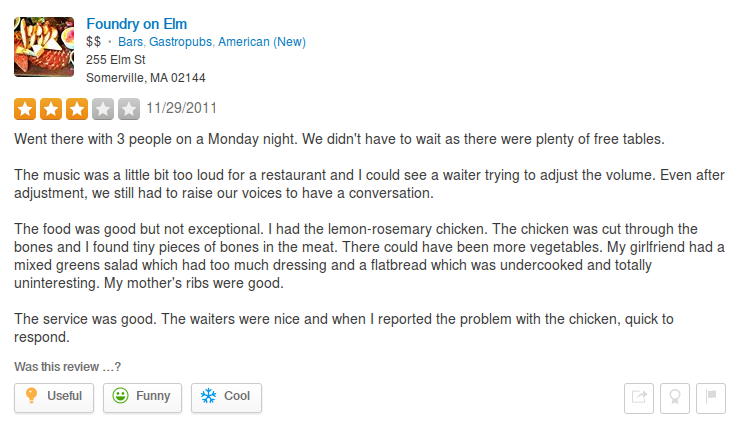
\includegraphics[width=12cm]{review_example.png}}
  \caption{Sample review with clearly expressed opinions.}
\end{figure}

This report introduces required theory, describes on a technical level accessible to computer scientists
not directly familiar with natural language processing how to develop a system that
mines opinions to produce comparable summaries. Included are also more detailed studies of a two concepts
shown to directly improve results: \emph{Smoothing} and \emph{down-sampling}.


% why group?
%The first and most important observation is that even if we find a statement and
%accurately identify it as a positive mention on something, it is not enough to merit a conclusion.
%Opinions are per definition subjective, and should individually be considered unreliable.
%However, as the number of processed opinions increase, so does confidence in conclusions that are based on them.
%
%As a consequence, four positive mentions of ``steak'' may not be enough for a conclusion,
%but in combination with positive mentions on ``chicken'', ``turkey'',  and ``meatballs''
%one may be able to conclude positive the common \gls{superword} \emph{meats}.
%Or if more confidence is required, ``salads'' may be included under
%the \gls{superword} \emph{food}, and so on.
%



\section{System overview}
This report introduces a system, which given a set of opinion-rich documents produces a summary of these
opinions, grouped by their \emph{opinion target} (the subject of the opinion)
and their \emph{semantic orientation} (positive or negative).

The goal for the produced summary is to contain everything required to draw conclusions about opinions
and to enable future work to create interactive visualizations.

To accomplish this, three tasks are introduced. This chapter will make a few definitions, and then go on to
describe each task briefly. Finally some shared theory will be introduced.



\section{Important definitions}

\subsubsection{Entity and its Aspects}
In this work, and often in sentiment analysis, \emph{entity} is used to mean the entity under review. But reviews are typically more detailed
and describe \emph{what} about an entity causes sentiment. An aspect of an entity, is used to mean \emph{what} about an entity is referenced.

E.g. in the sentence \emph{``my camera is very reliable''} the reviewed entity is \emph{camera} and the reviewed aspect is its \emph{reliability}.

Readers should be aware that older literature may refer to aspects as \emph{features}, which was changed with increased application of machine learning methods in sentiment analysis, to avoid confusion with \emph{features} in machine learning contexts.

\vspace{1cm}

\subsubsection{Opinion}
\emph{Liu} (2012) introduces \emph{opinion} as $(e_i,a_{ij},s_{ijkl},h_k,t_l)$-quintuples\footnote{Subscripts are
  used to indicate dependencies between tuple elements.},
where $e_i$ is the entity the opinion is referencing,
$a_{ij}$ is the aspect of $e_i$ that is being referenced (e.g. for a restaurant its ambiance),
$s_{ijkl}$ is the sentiment of the opinion,
$h_k$ is the opinion holder and
$t_l$ is the time of the experience the opinion is based on\cite[Chapter~2.1]{liu2012sentiment}.

In this work, the reviews used enable a few simplifying assumptions:
\begin{itemize}
\item The opinion holder $h_k$ is the logged in user posting the review.
\item The time $t_l$ is the time the review was posted.
\item The entity $e_i$ is the one for which the review is being posted.
\end{itemize}

%todo discuss assumption consequences?
Thus in this report, an opinion can generally be thought of as a $(a,s)$-tuple; or in plain words, an aspect with associated (non-neutral)sentiment.
\vspace{4cm}

\pagebreak

\section{Introduction of tasks}
Solutions to the following three tasks will be the basis for our system.
Below they are briefly introduced with the most important findings in this work and references
to subsequent chapters, where they are studied individually and in more detail.

The reader is advised to look at figure \ref{fig:overview}; which aims to
give an overview of how the tasks relate to one another.

\subsection{Aspect extraction}
Before anything else can be done, opinions need to be found and extracted from documents.
This is studied in chapter \ref{sec:aspect_extraction}, where the task is described in more detail,
and a simple solution is introduced.

The introduced solution is shown to achieve somewhat mediocre results, but estimates indicate
that results may be sufficient for big data sets.

Finally consequences of using a simple method are discussed, and a few improvements suggested in literature
to use in case data is limited are introduced.


\subsection{Sentiment classification}
Sentiment classification is the task of deciding whether sentiment in text is positive, negative or neutral.

Chapter \ref{sec:sentiment_classification} introduces \ngram~language models and how they can be used
to classify sentiment. \emph{Smoothing} is also introduced studied in depth in this section.

Good results are achieved, and it is shown that smoothing can significantly increase language
model performance.

\subsection{Aspect grouping}
In this work, aspects are grouped to enable comparisons between businesses that may not have exactly the same aspects ---
for example it is perfectly reasonable to compare a taco restaurant with a burger joint using the aspect group \emph{food}
if opinions on various tacos and burgers are assigned that group.

Chapter \ref{sec:aspect_grouping} introduces and compares two methods of grouping aspects into predefined groups;
one supervised and one algorithmic. This chapter also studies data bias and its consequences more carefully,
and results confirm that machine learning classifiers are indeed susceptible to data bias.

Results also show that the algorithmic classifier outperforms machine learning methods,
but also that machine learning methods are very likely to benefit from more training data,
and several concerns about the algorithmic method are raised.
Based on that the supervised machine learning method is recommended over the algorithmic one.


\begin{figure}[t]
  \centering
  \fbox{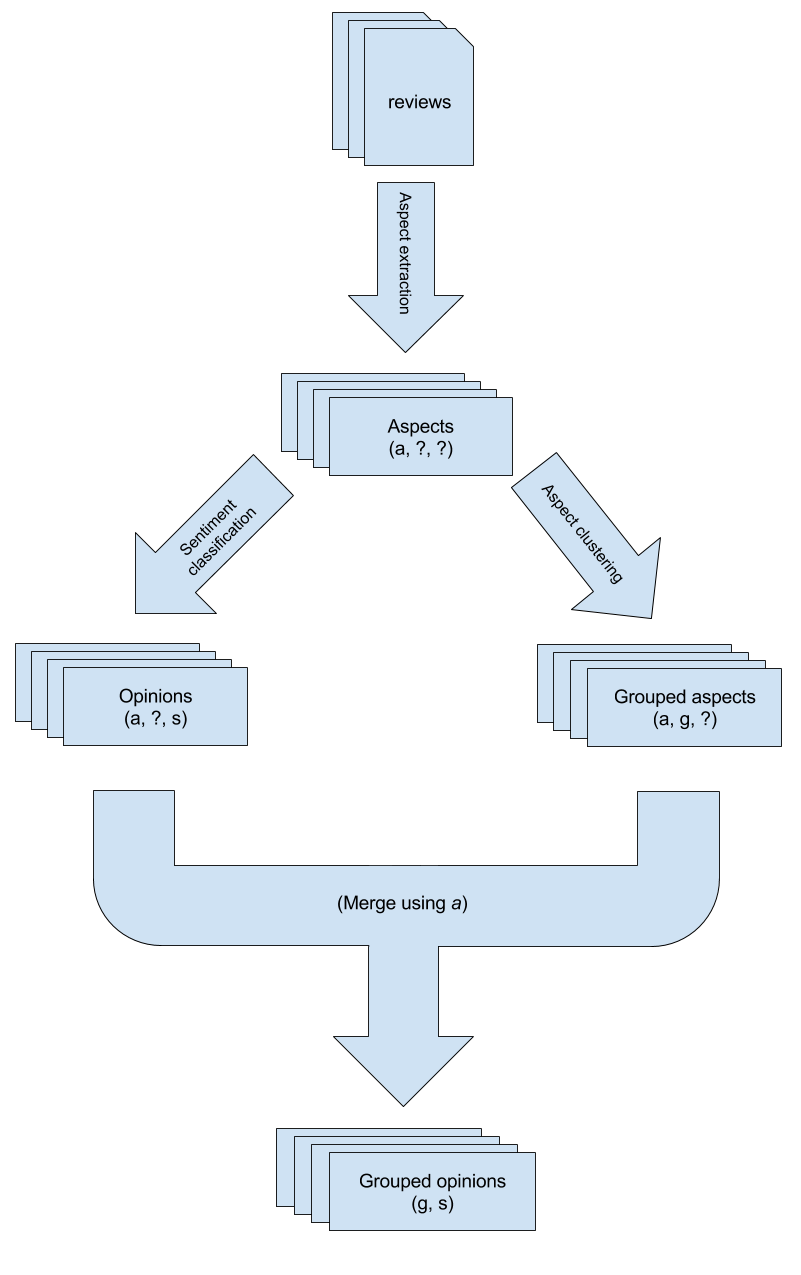
\includegraphics[width=12cm]{overview.png}}
  \caption{High level system overview. Unprocessed review texts processed by the system
    get turned into Grouped opinions; which are partial }
  \label{fig:overview}
\end{figure}



\clearpage

\newpage
\section{Levels of sentiment analysis and this work}
Sentiment analysis, the field of study under which opinion mining falls,
is typically divided into three levels of granularity:

On the \emph{document-level}, an entire review would be classified for
its overall-sentiment value\cite[Chapter~1.2]{liu2012sentiment}.
Although this may introduce difficulties with different sentiments
and largely varying document lengths, the fact that the document-level usually holds more information
means it is usually slightly simpler than the other levels.

The \emph{sentence-level} can still hold contradicting sentiments,
\emph{e.g. ``I love this restaurant even though the service is terrible''},
but this risk of multiple sentiments that are different is smaller in sentences
since they are shorter than full documents.

To fully address the issue identifying exactly what people liked,
sentiment classification has to be done on the \emph{aspect-level}.
On this level, sentiment has to be liked to an identified aspect in order to be considered
useful, which makes it much more useful, but also significantly increases complexity\cite[Chapter~1.2]{liu2012sentiment}.

The Yelp reviews used in this work are already assigned an overall rating towards the entity under
review, which is what sentiment analysis on the document-level would have resulted in.
Therefore, in terms of the above, this work applies a combination of sentence-level and aspect-level
sentiment analysis:

Aspects are extracted and grouped on the aspect level, and sentiment classification is done on
the sentence-level. This is done by assigning the average sentiment of the full sentence they appear in,
which may seem as an intrusive simplification, which is why it is
further discussed and motivated in section \ref{subsec:sentence_contradictions}.



%\subsection{Perplexity}




\chapter{Aspect extraction}

Aspect extraction is the task of finding and outputting sentiment carrying expressions
with identified \emph{targets}. A target is either some aspect of the entity that is
subject to the sentiment, or the entity in its entirety. E.g. in the sentence
\emph{``I like \textbf{this place} even though \textbf{the service} isn't great''},
there are two opinions with one (highlighted) target each; the entity itself, and the
service-aspect of the entity.

Aspect extraction then is a typical information retrieval task, and thus methods
(including evaluation) can be recognized from data mining- and other information retrieval tasks.
In general, there are four approaches to aspect extraction\cite[chapter 5.3]{liu2012sentiment}:

\begin{enumerate}
\item Extraction based on frequent nouns and noun phrases
\item Extraction by exploiting opinion and target relations
\item Extraction using supervised learning
\item Extraction using topic modeling
\end{enumerate}
This work mainly employs the first kind, with some of pruning methods defered to
later tasks using supervised learning (further details in section
\ref{subsec:pruning}).

Results will show it sufficiently effective to not examine other methods in
this work.

\subsection{A data dependent task}
Like other data extraction tasks, aspect extraction is largely dependent on the data
aspects are being extracted from; meaning techniques may vary in effectiveness depending
on what domain they are applied to, demographics of review authors,
contextual expectations of the reviewed entity and countless other factors.

Furthermore, even within the same data set, there may be hidden properties on a
per-entity basis. E.g. one could imagine that even on the same review site, there would still
be systematic differences between reviews written for a surgeon's instrument
compared to reviews for a toy car.

It is therefore crucial that in the process of aspect extraction, like in other extraction tasks,
to think about what correlations may exist and what bias they may introduce in the extracted data.


\subsection{Candidate extraction vs. pruning}
There are two important definitions in this section,
which together make up the method used in this work:

\emph{Candidate identification} is the task of finding potential aspects in unstructured text.

\emph{Pruning} is the task of excluding irrelevant candidates that from the candidate
identification result set.

The reason why these usually are done separately in sequence is that many common pruning
techniques require the full candidate set when deciding whether to prune.
(Examples include \emph{idf}-scores or plain occurrence counts.)


\section{Related Work}

\subsubsection{Turney (2002)}
In early work, Peter Turney classified sentiment of reviews for \emph{automobiles}, \emph{banks}, \emph{movies} and \emph{travel destinations} with accuracies ranging from 66-84\%, by extracting aspects using predefined POS-patterns, and querying search engines for the co-occurrence between found patterns and the words \emph{``excellent''} and \emph{``poor''}.

\subsubsection{Hu, Liu (2004)}
In ``Mining Opinion Features in Customer Reviews'' aspects are unsupervisedly
extracted by considering frequent noun phrases found in data using POS-tagging.

This approach appears to return a lot of false positives, which is why two pruning
methods are introduced to improve precision.

Sentiment classification is also mentioned, but those results are presented in a subsequent paper.

\subsubsection{Liu, Hu and Cheng (2005)}
In ``Opinion observer: analyzing and comparing opinions on the web'', their previous work is extended
by a visualization interface and a more sophisticated method of aspect extraction is introduced.

In short, their extraction is done the following way:

Sentences are split into segments (using dots, commas, conjunctions etc.), POS-tagged, and aspects are
manually replaced by tokens. Sentences are then broken into unordered \emph{trigrams},
and words not replaced by tokens are stemmed.

Finally, \emph{association rule mining}\cite{ma1998integrating} is used to find implications
from either words or word-classes to those aspect tokens.

%For an example, consider the sentence \emph{``I like the easily used autofocus''}.
%\emph{autofocus} is annotated as the aspect  andthe rest of the sentence is stemmed,
%resulting in something like: \\
%``\texttt{<PRP>}\emph{I} \texttt{<VB>}\emph{lik} \texttt{<DT>}\emph{the} \texttt{<JJ>}\emph{easy}
%\texttt{<VB>}\emph{us} \texttt{<NN>}<aspect>''.
%
%One of the trigrams found above (\texttt{<JJ>}\emph{easy}, \texttt{<VB>}\emph{us}, \texttt{<NN>}<aspect>)
%would increase confidence in rules like \{\emph{easy}, \texttt{<VB>}\} $\rightarrow$ <aspect> amongst others.




\section{Extracting aspects}
\subsection{Candidate Identification}
A simple aspect extractor was developed. Given a review, much like Turney's pattern extraction,
the extractor uses the POS-tagger in nltk\cite{nltk} and
compares text to a series of predefined grammatical patterns.

These patterns were acquired during the annotation described in section \ref{subsec:getting_data},
where each annotated aspect also included its POS-pattern. As happens to be, all patterns match noun-phrases.

A total of 511 unique patterns were found, but out of those, the 33 that occurred more than
once were examined. Out of those, 6 patterns were removed since they were two words or shorter
and visual inspection of results indicated they produce significantly more false positives.

The remaining patterns which were used are listed in table \ref{tab:used_pos}.

The extractor uses the first pattern that matches, which then ``consumes'' that part of the text.
Therefore, patterns were ordered by length to make sure that the longest possible pattern
matches, and within the same length the order was determined by
the number of times the pattern occurred in the annotated data.

One more observation was made: Several patterns have (some version of) the same word-class,
examples include the \texttt{<PRP><VBZ><JJ><JJ>} and \texttt{<JJ><NN><NN>} patterns.
This also aligns well with understanding of the English language, where several nouns in sequence,
like ``tooth brush'', usually still represent only one entity, and thus does not change
the meaning of the pattern itself.

With this in mind, an experiment was set up where patterns were extended to allow
multiple words of same word-class in sequence wherever a noun(\texttt{<NN>+})
or adjective(\texttt{<JJ>+}) occurred.
This experiment is called \texttt{Modified patterns} in the results, as opposed to
the original \texttt{Unmodified patterns}.

\subsection{Pruning}
\label{subsec:pruning}
The only pruning applied in this work comes as a side effect of the methods introduced
in the other two chapters, sentiment classification and aspect grouping, and the
confidence thresholds that they allow.

In both chapters, confidence thresholds are introduced as a means of increasing
precision at the cost of recall, and the aspects that fall under the confidence threshold
are effectively being pruned. Please note that results in this chapter are presented
before any pruning has been done, as the pruning process is intimitely related
to the other two tasks.

%In section \ref{subsec:suggested_pruning} pruning methods are discussed further.

\subsection{Evaluating extraction performance}
% todo
Information retrieval tasks are often evaluated with two capabilities in particular
in mind, namely the capabilities of excluding irrelevant results and including relevant ones.
These are formally introduced later as \emph{precision} and \emph{recall} in
section \ref{sec:precision_recall}, but for this section an informal definition should be sufficient.

The way tasks are divided in this work, with further pruning subsequently done in
the later tasks, one of the most important questions for aspect extraction is
\emph{will it find enough candidates to for a reasonable summary?}

Therefore, 




\newcommand{\ExtrPatOne}{\texttt{<NNS?><VB.?>+<JJ.?>+}}
\newcommand{\ExtrPatTwo}{\texttt{<NNS?><VB.?>+<RB.?><JJ.?>}}

\begin{table}[t]
  \centering
  \begin{tabular}{| l | c | l |}
    \hline
    \textbf{Pattern} &\textbf{No.} & \textbf{Sample sentence} \\ \hline
    \texttt{<DT><NN><VBZ><RB><JJ><CC><JJ>} & 2 & \emph{``The staff is very good and friendly''}\\
    \texttt{<DT><NNS><RB><VBP><RB><JJ>} & 2 & \emph{``The people here are very friendly''}\\
    \texttt{<PRP><VBZ><RB><DT><JJ><NN>} & 2 & \emph{``It is always a little dirty''}\\
    \texttt{<DT><NN><VBD><RB><RB><JJ>} & 2 & \emph{``The food was not sloppily prepared''}\\
    \texttt{<DT><NN><VBZ><RB><RB><JJ>} & 2 & \emph{``The pizza is still really good''}\\
    \texttt{<DT><NN><VBZ><RB><JJ>} & 11 & \emph{``The place is immaculately clean''}\\
    \texttt{<DT><NN><VBD><RB><JJ>} & 2 & \emph{``This dessert looked pretty good''}\\
    \texttt{<DT><NNS><VBP><RB><JJ>} & 2 & \emph{``The prices are not bad''}\\
    \texttt{<DT><NN><VBD><JJ>} & 9 & \emph{``The bread was horrible''}\\
    \texttt{<PRP><VBD><RB><JJ>} & 4 & \emph{``He was extremely rude''}\\
    \texttt{<DT><NN><VBZ><JJ>} & 4 & \emph{``The location is great''}\\
    \texttt{<IN><DT><JJ><NN>} & 3 & \emph{``At a fair price''}\\
    \texttt{<DT><NNS><VBD><JJ>} & 3 & \emph{``The facilities were clean''}\\
    \texttt{<PRP><VBZ><JJ><JJ>} & 2 & \emph{``It 's metro accessible''}\\
    \texttt{<NN><VBD><RB><JJ>} & 2 & \emph{``Everything was very delicious''}\\
    \texttt{<NN><VBZ><RB><JJ>} & 2 & \emph{``Restaurant is very clean''}\\
    \texttt{<PRP><VBP><JJ><NNS>} & 2 & \emph{``They have sweet booths''}\\
    \texttt{<DT><NNS><VBP><JJ>} & 2 & \emph{``The salads are fresh''}\\
    \texttt{<JJ><NN><NN>} & 6 & \emph{``Great clam chowder''}\\
    \texttt{<RB><JJ><NN>} & 4 & \emph{``Sloppily prepared sandwich''}\\
    \texttt{<NNS><VBP><JJ>} & 3 & \emph{``Portions are huge''}\\
    \texttt{<JJ><JJ><NN>} & 3 & \emph{``Consistent excellent quality''}\\
    \texttt{<PRP\$><JJ><NN>} & 3 & \emph{``Their amazing vinaigrette''}\\
    \texttt{<NNP><JJ><NN>} & 3 & \emph{``Great Italian food''}\\
    \texttt{<JJ><JJ><NNS>} & 3 & \emph{``Fresh generous subs''}\\
    \texttt{<JJ><VBG><NN>} & 2 & \emph{``Tasty looking food''}\\
    \texttt{<RB><RB><JJ>} & 2 & \emph{``Admittedly not cheap''}\\
    \hline
    \textbf{Excluded patterns} && \\
    \hline
    \texttt{<JJ><NN>} & 24 & \emph{``Good food''}\\
    \texttt{<JJ><NNS>} & 7 & \emph{``Reasonable prices''}\\
    \texttt{<NNP><NN>} & 5 & \emph{``Great food''}\\
    \texttt{<NN><NNS>} & 3 & \emph{``Singing waiters''}\\
    \texttt{<NN><NN>} & 2 & \emph{``Bland food''}\\
    \texttt{<RB><VBN>} & 2 & \emph{``Reasonably priced''}\\
    \hline
  \end{tabular}
  \caption{Patterns found when annotating and how frequent they were.
    For a complete list of the word classes used in the patterns, see Appendix \ref{TODO}.
  }
  \label{tab:used_pos}
\end{table}

\begin{sidewaysfigure}[h]
  \centering
  \begin{tikzpicture}

  \begin{axis}[
      xlabel={Aspects found in review},
      ylabel={No. reviews},
      ybar, ymin=0, %3ymax=9999,
      bar width=6pt,
      xtick=data,
      x=0.8cm,
      xmax=23,
      enlarge x limits={abs=0.5cm},
      %x tick label style={rotate=45,anchor=east},
      xticklabels from table={data/extraction_count_all_modified.csv}{found},
      xticklabel style={text height=1.5ex},
      ymajorgrids=true,
      grid style=dashed,
      legend pos=north east,
    ]
    \addplot table [x expr=\coordindex, y=count]{data/extraction_count_unmodified.csv};
    \addplot table [x expr=\coordindex, y=count]{data/extraction_count_all_modified.csv};
    %\addplot table [x expr=\coordindex, y=count]{data/extraction_count_both.csv};
    \legend{
      \hspace{0.4cm}\texttt{Unmodified patterns},
      \texttt{Modified patterns}
    }
  \end{axis}
  \end{tikzpicture}
  \caption{Distribution of how many aspects were found in  reviews.
    The height of each bar represents in how many out of 10'000 reviews exactly $n$
    aspects were found, where $n$ is the column of the bar. Thus, each bar represents
    $n$ times as many aspects as its height. E.g. the second column, with just over 1,600
    reviews, represents twice as many aspects.
  }
  \label{fig:extr_count}
\end{sidewaysfigure}

\clearpage

\section{Results}

Out of 10'000 reviews, a total of 27'656 aspects were found using the modified patterns
and 26'766 using the original patterns.
Figure \ref{fig:extr_count} shows the distribution of reviews and the number of
found aspects. The figure has been cut at 21 reviews, but two reviews had as many
as 22 and 23 aspects found in them, respectively.

Note that the graph does not show how many aspects were found,
but in how many reviews a certain number of were found, which means that for the
total sum each count has to be multiplied with the number of aspects it corresponds to.

\section{Discussion}
\subsection{The modified patterns}
As results show, there is very little difference between the modified patterns and
the original ones. Although the modified patters do find a few more aspects, looking
at the distribution in figure \ref{fig:extr_count} the additional aspects more often
appear to be found in reviews where aspects were already found, or in other words;
the modified patterns appear to further favor the writing styles of already included authors.

In fact, out of the 110 new aspects found, only 5 aspects came from new reviews.
On the other hand, I believe there is marginal downside to keeping these modified
patterns after glancing over the additional aspects, but without a quality measure
it is hard to definitely tell. 

\subsection{Aspect quantity}
On average, around 2.7 aspects per review are found, which may not sound like a lot 
but for entities with lots of reviews it is enough:

Later in this work when aspect clustering is studied, figure \ref{fig:cat_count}
will show that the least common category, \emph{value}, represents around
10\% of all aspects.

Glancing at future results, confidence thresholds with $recall\approx 0.7$
appears reasonable for both sentiment classification and aspect grouping.

An estimate for the number of value aspects found for a business with 300 reviews
using the numbers in this section is $300 \cdot 2.7 \cdot 0.7^2 \cdot 0.1 = 39.69$ aspects.
Around 40 aspects should be enough to give a statistically significant indication.
Especially as in practice review comparisons are likely going to be done for
business chains which can have 10'000 reviews or more.

\subsection{Evaluation of aspect extraction}

%todo rewrite

The results in this section are a bit vague, but there is a reason for this.
Common practice in information retrieval is to use precision as a measure of
quality, however, this requires a clear definition of what is relevant.
When manually annotating aspects I found it difficult to determine where to draw the
line for what an aspect is. As section \ref{subsec:objective_sentiments} describes,
sentiments can be derived from various forms of sentences.

My concern was that what definition I decided upon would influence the results without
reflecting the methods effectiveness.

Thus, I decided to revisit metrical measures when I aspect extracting became the
bottleneck of the systems performance, which is a point I never reached in this work.

I believe it could be a good idea to evaluate aspect extraction in the context of
the full system and not individually, as what to extract is so dependent on what
the purpose of the extracted data is. This would probably also make it easier to
determine what is relevant and what is not.

\subsection{Mitigating author bias}
76 review out of 10'000 had more than 13 aspects with one review having as much as 23 aspects.
If we simply included each aspect from reviews like that one the opinions of
those sole authors would be represented 23 times more than the opinions from reviews
with one extracted aspect each.

Luckily, a simple way to make conclusions more impartial is to only allow one
opinion per aspect group from each review.
I.e. each review contributes with \emph{at most} one opinion on product, one on service, etc.
The opinion should be picked so that it represents the majority of
sentiments expressed towards that aspect group.

The results in this section do not have the aspect groups associated with them,
but an absolute lower bound to how many aspects can be kept in the worst case
is found by simply discounting all but one aspect from each review. This is the same
as summing the counts of all non zero bars in figure \ref{fig:extr_count}, and the
exact sum is 7851, or equally 7.85\% of reviews.

That being said, it is probably OK and even preferred to allow a few more opinions per review,
but an upper limit can make sure that a one or a few rigged reviews will not compromise results.


\section{Further work}
\subsection{Further mitigating author bias}
I believe it to be more important to reduce the number of reviews where no aspect was
found at all. My current results where at least one aspect is found in approximately
80\% of reviews are decent but could be improved.

This is desired to mitigate bias towards or against authors writing with certain styles.
However, in pursuit of this, I would advice to use more metrics; either annotated data
or at least metrics normalized by review length. I suspect that some in some cases
aspects are not found because reviews are really short and/or because there are no aspects
to find.

\subsection{Named Entity pruning}

Something I have come across and which should be pruned is mentions of other businesses
in reviews. A sentence like
\emph{``I recommend this place over Alfredo's across the street, because their pizza tastes like rubber.''}
, although perfectly reasonable in a review, will inaccurately discredit
the evaluated business for its neighbour's rubber-like pizza.

Pruning these mentions should be reasonably simple using \emph{named entity extraction}, where named
entities found could be compared to the name of the business under review and if not matching,
the sentence along can be then be pruned.

As a bonus, named entities that are found to refer to the business can be replaced
with a token value which likely will improve performance of language models in future chapters.

%patterns by reinforcement learning?

% the word 'and'
% noun-phrases
% couting patterns i.e. a, b, c, and/or d

%%%%%%%%%% toss comparing opinions and NE

\chapter{Aspect Grouping}
Thus far this work has introduced methodology for extracting aspects from text.
Recall from the last chapter that aspect extraction yields noun phrases that are likely
to hold an opinion.
Identifying the aspects of these opinions is a key task as it is what enables
summaries about \emph{what} opinions actually are about, rather than treating all opinions
as sentiments about the reviewed entity in its entirety.

To illustrate, imagine an entity with a mix of positive and negative opinions.
Without identifying what aspects of the entity the opinions are targeting, the best
you can do is averaging the positive with the negative.
Whereas if the aspects were identified 
it would be possible to find out what in specific is the cause of opinions;
one might find some aspects to be cause of consistently positive or negative opinions,
or one may find aspects with disagreeing oppinions
--- either discovery is likely to be highly useful!

\subsection{Why group aspects?}
Identifying aspects is not enough. Finding that the
most appreciated aspects of a restaurant are \emph{french fries},
\emph{fried potatoes}, and \emph{fries} is superfluous as they are
clearly referring to the same thing.
This could potentially be a problem for aspects that are very diversely described;
to ensure reliability and counteract subjectivity, aspects with few opinions are
likely to be ignored, so there is a risk valuable opinions are disregarded unless
mulitple descriptions of the same aspect are grouped as one. This is known as \emph{synonym grouping}.

%todo group tree figure

It may be beneficial to take this grouping even further;
if there after the grouping still are too few opinions about \emph{fries},
it might be possible to further group with opinions about \emph{mashed potatoes}
and \emph{baked potatoes} under the shared (hyopnymIteratively \emph{potatoes} can
be grouped with \emph{salads} as \emph{sides} and so forth with each iteration aggregating
more opinions under the same label.

This has another important side effect; it enables comparisons that would otherwise
be impossible, becasue to compare two entities they need shared aspects.
E.g. when comparing an italian restaurant and an asian restaurant, sufficient aspects may
have been found for \emph{pasta carbonara} and \emph{vegetable wok}, but neither of
those aspects is shared by both entities, rendering comparison is impossible.
However, if aspects are grouped under a shared hyponym, such as \emph{main courses},
the entities can be compared using this common aspect.


\subsection{Aspect grouping in this work}
%todo

\section{Grouping methodologies}
\subsection{Lexical graph search}
Based on the observation that there are usually keywords in a sentence with lexicographical connection to the desired category, an alternative approach to traditional classification is proposed. This is motivated since classification models need pure training data to achieve good results. The idea is to use a lexicon of known word relations to find a path from a query word to one of few word senses with predefined category label, and assign the query word the same label.

Figure~\ref{fig:baklava_lex} shows an example of this premise in action, where the word relations involved in finding the word ``baklava'' were used, and that it is closer to \emph{product} than \emph{establishment}.

\subsubsection{The algorithm}
A \gls{BFS}(BFS) is conducted from the initial category word senses, defined in table \ref{cat_words}. For each word, neighboring word senses are acquired using word relations defined by \gls{jaws}). Each word sense is also mapped to its source category in this process to allow for quick look-ups.

This method to categorize individual words, can then be extended to categorize full sentences using heuristics.

\subsubsection{Voting heuristic}
The heuristic is what actually classifies sentences into groups. To do this, it can use the above described group to query for the group of an individual word sense. Since word senses can consist of more than one word, e.g. ``happy hour'', the heuristic iteratively searches for multiple word word-senses, decreasing in length, starting with the assumption that the full sentence is one word.

Next, a map is built using enabling constant time lookup of not only which group is nearest,
but also the distance $d$ from the word sense to the category.

This is then combined into one score using the following scheme:

\begin{equation} \label{eq:heruistic}
  category(s) =
  \underset{k}{\text{argmax}}
  \sum_{w \in s} categoryScore(w, k)
\end{equation}

\begin{equation} \label{eq:heruistic_d}
  categoryScore(w, k) =
  \begin{cases}
    max(d_*) - d_k(w) + 1, & \text{if}\ k \text{ is the nearest class}\\
    0, & \text{otherwise}
  \end{cases}
\end{equation}

where $d_k(w)$ is the distance from the word sense $w$
to its nearest category and $d_*$ is the highest distance any word in the sentence
has to its nearest category(making the category score for worst scored word in the sentence 1).

This way, for a three word sentence $s=w_1w_2w_3$ with the nearest distances
$d_A(w_1)=4$, $d_A(w_2)=6$ and $d_B(w_3)=3$,
the categories will receive the scores $A=3+1+0$ and $B=0+0+4$, and the highest scoring category $A$
would be selected.

\begin{table}[t]
  \centering
  \begin{tabular}{| c | c |}
    \hline
    \textbf{Category} & \textbf{Predefined keywords}\\ \hline
    Establishment & \emph{Furniture, view, music, loud, appearance, clean, location}\\ \hline
    Product & \emph{food, drink, taste, edible}\\ \hline
    Value & \emph{Cheap, price, dollar, buck, lots, bargain}\\ \hline
    Service & \emph{Service, quick, attentive, wait}\\ \hline
  \end{tabular}
  \caption{Categories with their pre-associated key words.}
  \label{tab:cat_words}
\end{table}

\begin{figure}[t]
  \centering
  \fbox{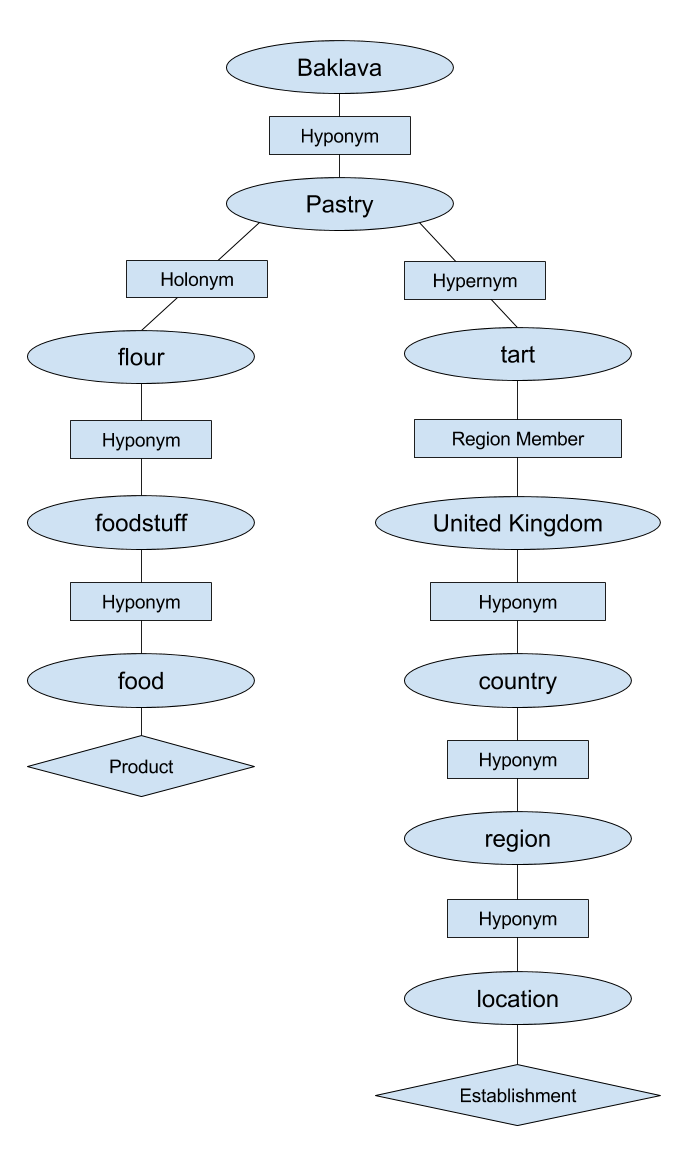
\includegraphics[width=10cm]{img/baklava_lex.png}}
  \caption{Example showing how ``baklava'' could be lexicographically closer to category ``product'' than ``establishment''. Ellipses represent word senses, rectangles the relations between senses, and diamonds predefined categories with a few associated senses (in this case \emph{food} and \emph{location}).}
  \label{fig:baklava_lex}
\end{figure}

\subsection{Machine learning classifiers}

\todo
warranted bias study

\clearpage

% todo: num sentences table


\section{Evaluation}
\label{sec:precision_recall}
A common way to evaluate information retrieval tasks is \emph{precision}
and \emph{recall}. Together they evaluate a systems ability to retrieve results,
by evaluating the capacity to exclude irrelevant results,
and include relevant results, respectively.

\subsection{Precision}
% todo: accuracy
Precision is a measure of what fraction of retrieved results are considered relevant or correct.

It is defined as follows:
\begin{equation} \label{eq:precision}
Precision = \frac{\text {correctly classified}}{\text{correctly classified} + \text{incorrectly classified}}
\end{equation}

\subsection{Recall}
In this work, confidence thresholds are used to examine whether better results can be achieved by
allowing the classifiers answer \texttt{UNKNOWN} for difficult cases. These answers are not included in
the precision denominator, as they are not considered to be classified.
Instead \emph{recall} is introduced to mean the fraction of results that classifiers gave an answer for:

\begin{equation} \label{eq:recall}
Recall = \frac{\text {classified}}{\text{classified} + \texttt{UNKNOWN}\text{s}}
\end{equation}


\newpage
\subsection{Getting data}
\label{subsec:getting_data}

\begin{figure}[h]
  \centering
  \fbox{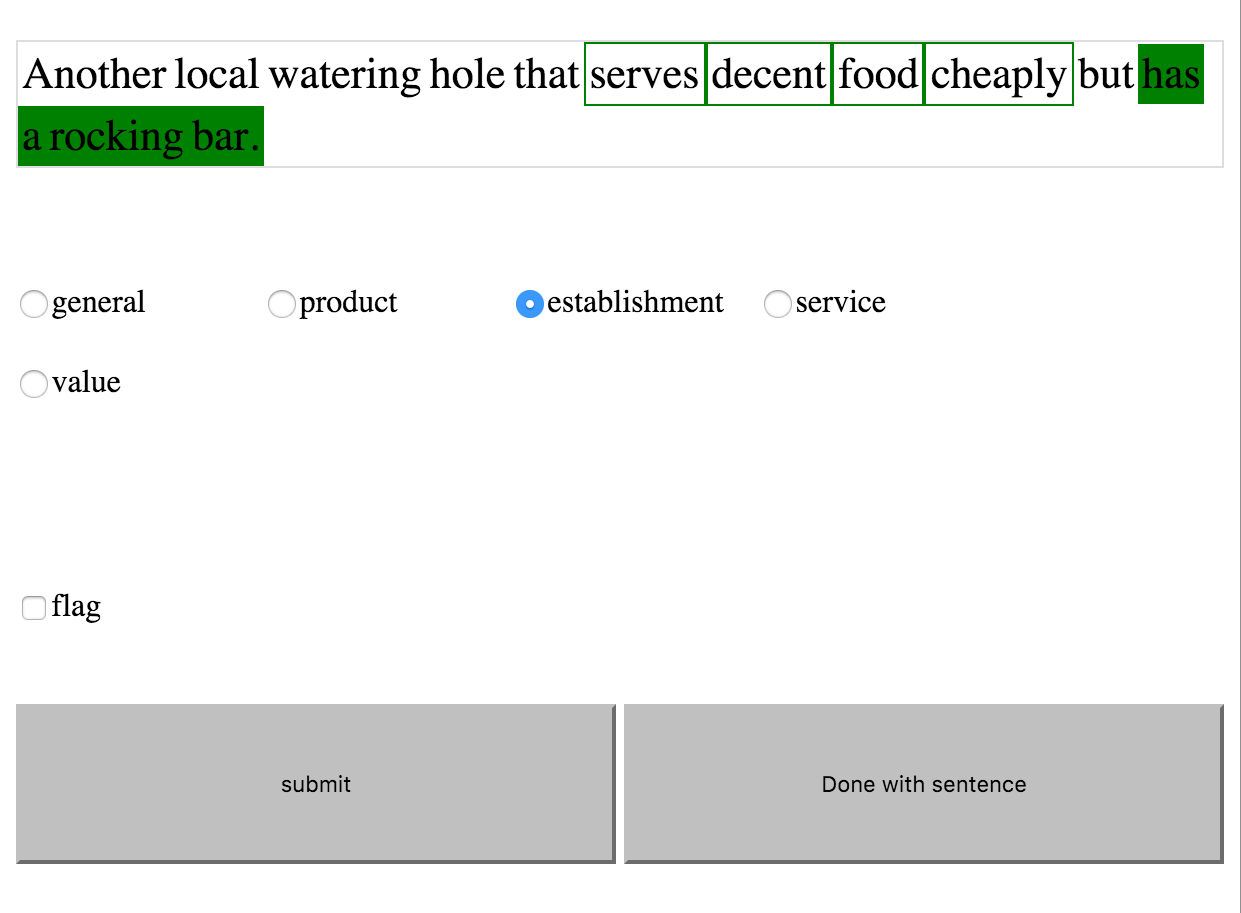
\includegraphics[width=10cm]{annotate_aspect.png}}
  \caption{Aspect level annotation interface. Allows selection of aspects by marking a series of words(dark green). Since a sentence can hold more than one aspect, once an aspect has been submitted, the same sentence is kept and another aspect can be selected(a green border is left to indicate a previous submission).}
  \label{fig:annotate_aspect}
\end{figure}

Figure \ref{fig:annotate_aspect} show the interface that was developed to annotate aspects
according to their group and sentiment.

This simple web-interface was served by a local web server.

\begin{figure}[t]
  \centering
  \begin{tikzpicture}

  \begin{axis}[
      %title={Classifier performance per category},
      %xlabel={Categories},
      ylabel={Number of aspects},
      ybar, ymin=0,
      %bar width=20pt,
      xtick=data,
      x tick label style={rotate=45,anchor=east},
      xticklabels from table={data/category_distribution.csv}{category},
      xticklabel style={text height=1.5ex},
      ymajorgrids=true,
      grid style=dashed,
      legend pos=north east,
    ]
    \addplot table [x expr=\coordindex, y=count]{data/category_distribution.csv};
  \end{axis}
  \end{tikzpicture}
  \caption{Number of annotated sentences per category}
  \label{fig:cat_count}
\end{figure}

\clearpage


\subsection{Skewed data}
\label{subsec:bias}
When dealing with real world data, it is possible that some classes in classification tasks are more
common than others. This has been shown to have consequences both in Bayesian classifiers\cite{rennie2003bias}
and Support Vector Machines\cite{svm_bias}, where both have been shown to favor majority
classes\cite{rennie2003bias, svm_bias}.


%todo 1/n
Not only classification methods, but also precision measures are affected by skewed data. In binary
classification with evenly distributed classes, a classifier that favors one class to the extreme that it
always chooses the same class, still achieves around 0.5 precision since the number of true positives
would equal the proportion of the favored class\footnote{This is in fact be the worst possible result
in the binary case, since any classifier performing consistently worse could be modified to return the
opposite and thus have the inverse precision which would be better.}.
If the evaluation data is also biased towards the same class, that classifier will get even
higher precision, which illustrates how important it is to examine classifier
bias and data distribution.

A commonly employed and simple way to solve problems with disproportionate data
is to exclude all but an equal amount from each class to artificially balance the class distribution,
more commonly referred to as \emph{down-sampling}\cite{provost2000machine}.
This could pose a problem if data is very skewed, as this means that the required
amount of available data effectively is divided by the fraction of the least common class.
However, in this work the data was not skewed enough to motivate studies of more
complicated approaches.

Although down-sampling eliminates bias in evaluations, which makes evaluations between
classifiers more comparable, it also reduces the amount of entries used in evaluations.
Therefore this report will evaluate using unscaled data once classifiers have been
verified to be reasonably unbiased in a per class comparison.



\section{Results}

This chapter is laid out as follows: First the individual results for each of the \numClassifierAproaches~classifier approaches are walked through. This gives the reader a chance to better understand section \ref{sec:comparison} where the classifiers are compared.


\subsection{Machine learning classifiers}

\begin{figure}[h]
  \centering

  \begin{tikzpicture}
    \begin{axis}[
        %title={Classifier performance based on data size},
        xlabel={Training data-set size},
        ylabel={Fraction of correctly classified},
        %xmin=0.3, xmax=0.7,
        %ymin=0.25, ymax=0.75,
        %xtick={0,20,40,60,80,100},
        %ytick={0,20,40,60,80,100,120},
        legend pos=north west,
        ymajorgrids=true,
        grid style=dashed,
      ]
      %\addplot table [x=n, y=p]{data/data_size_unigram.csv};
      \addplot table [x=n, y=p]{data/data_size_unigram_balanced.csv};
      \addplot table [x=n, y=p]{data/data_size_bigram.csv};
      \legend{
        %biased unigram,
        unigram,
        bigram
      }
    \end{axis}
  \end{tikzpicture}
  \caption{Sentence classification performance based on training data size}
  \label{fig:data_size}
\end{figure}


As expected, figure \ref {fig:data_size} shows that increased quantities of training data quickly yield improved results. This increment appears approximately linear, up to some point where it is expected to converge. Interesting is how the simpler unigram method quickly outperforms the bigram model, but that the bigram model sees very steady increment.

\pagebreak

\subsection{Per class classification}
\begin{figure}[h]
  \centering
  \begin{tikzpicture}

  \begin{axis}[
      %title={Classifier performance per category},
      %xlabel={Categories},
      ylabel={Fraction of correctly classified},
      ybar, ymin=0,
      %bar width=20pt,
      xtick=data,
      x tick label style={rotate=45,anchor=east},
      xticklabels from table={data/per_category_unigram.csv}{n},
      xticklabel style={text height=1.5ex},
      ymajorgrids=true,
      grid style=dashed,
      legend pos=north east,
    ]
    \addplot table [x expr=\coordindex, y=p]{data/per_category_unigram.csv};
    \addplot table [x expr=\coordindex, y=p]{data/per_category_unigram_unbalanced.csv};
    \addplot table [x expr=\coordindex, y=p]{data/per_category_bigram.csv};
    \addplot table [x expr=\coordindex, y=p]{data/per_category_bigram_unbalanced.csv};
    \legend{Down-sampled unigram, Unmodified unigram, Down-sampled bigram, Unmodified bigram}
  \end{axis}
  \end{tikzpicture}
  \caption{Down-sampled vs. not down-sampled classifier comparison. No confidence threshold was set in this experiment: recall was 1.}
  \label{fig:per_cat}
\end{figure}


%\begin{figure}[h]
%  \centering
%  \begin{tikzpicture}
%
%  \begin{axis}[
%      %title={Classifier performance per category},
%      %xlabel={Categories},
%      ylabel={Fraction of correctly classified},
%      ybar, ymin=0,
%      %bar width=20pt,
%      xtick=data,
%      x tick label style={rotate=45,anchor=east},
%      xticklabels from table={data/per_category_unigram.csv}{n},
%      xticklabel style={text height=1.5ex},
%      ymajorgrids=true,
%      grid style=dashed,
%      legend pos=north east,
%    ]
%    \addplot table [x expr=\coordindex, y=p]{data/per_category2_unigram.csv};
%    \addplot table [x expr=\coordindex, y=p]{data/per_category2_bigram.csv};
%    \legend{balanced unigram, unbalanced unigram, balanced bigram, unbalanced bigram}
%  \end{axis}
%  \end{tikzpicture}
%  \caption{Percat2}
%  \label{fig:per_cat}
%\end{figure}

Section \ref{subsec:bias} introduced bias in data, along with some of its
consequences which motivated a more detailed study of classifier results on
a per class basis. Figure \ref{fig:per_cat} illustrates how classifiers trained on
down-sampled training data perform much more consistent between classes.

Comparison between the balanced/unbalanced versions of the classifier models show that, as expected, there seems to be bias towards the more frequent $product$-class and respectively against the infrequent $value$-class.

It can also be seen that the bigram model is performing poorly for all labels except the \emph{product} class, but the reader is urged to note that this is a consistency between the balanced and unbalanced version of the model.

\newpage

\subsection{Introducing confidence thresholds}
\begin{figure}[h]
  \centering
  \begin{tikzpicture}
    \begin{axis}[
        %title={Classifier performance based on data size},
        xlabel={Recall},
        ylabel={Precision},
        %xmin=0.5, xmax=1,
        %ymin=0.4, ymax=1,
        %xtick={0,20,40,60,80,100},
        %ytick={0,20,40,60,80,100,120},
        legend pos=south west,
        ymajorgrids=true,
        grid style=dashed,
      ]
      \addplot table [x=r, y=p]{data/pr_unigram.csv};
      \addplot table [x=r, y=p]{data/pr_bigram.csv};
      \legend{
        unigram,
        bigram
      }
    \end{axis}
  \end{tikzpicture}
  \caption{Precision vs. recall created varying a confidence threshold}
  \label{fig:pr_curve}
\end{figure}


Figure \ref{fig:pr_curve} shows the expected precision/recall trade-off for the aspect cluster classifiers. Readers should be reminded that each measurement was done on differently balanced training data, which likely accounts for inconsistencies in the curves.

\newpage

\section{Graph-search classifier}
%todo NUM X
The graph search found and categorized a total of 78'844 word senses, and as a reminder,
these words are labeled solely using the $X$ predefined words from table \ref{tab:cat_words}.

%todo notable failures?

\section{Comparison of classifiers}
\label{sec:comparison}

\begin{table}[h]
  \centering
  \pgfplotstabletypeset[
    columns={method,p,r},
    col sep=comma,
    every head row/.style={after row=\midrule},
    columns/method/.style={string type,column type=l, column name=Classifier},
    columns/p/.style={precision=3, column type=l, zerofill, column name=Precision},
    columns/r/.style={precision=4, column type=l, column name=Recall},
  ]{data/general_aspect.csv}

  \vspace{0.4cm}\caption{Result summary}
  \label{general_asp}
p\end{table}


\section{Discussion}
\subsection{Graph search classifier}
As the results show, it is in fact possible to categorize aspects using a lexical database.
What is particularly interesting about this result is that, although the method is evaluated in a supervised
manner, the heuristic is in itself unsupervised. %todo retrofit for hillclibming?


The origins of this method are largely narrated by the introductory section of this chapter;
when getting the system to work initially, aspects were merely grouped by their lemmatized rightmost noun.
This introduced an obvious need for \emph{synonym grouping}. Later, when studying this task in more detail,
this method was evolved retrofitting the existing solution with further WordNet word relations.

\subsection{Machine learning classifier}

\subsection{Comparision}

\subsection{Conclusion}

There are however a few reasons why the results should be interpreted with caution:

I believe my limited amount of data to have much influence over my results.
As figure \ref{fig:data_size} illustrates, neither machine learning classifier
appears ``saturated'', and would most likely have benefited from more annotated aspects.

Another important thing to keep in mind about my results are that with such a small data-set,
there is a risk of methods becoming too specific toward the training data.
This is often discussed in statistical modeling as \emph{``overfitting'' },
but the same phenomenon can also appear with heuristics.
I believe that some aspects of my data make this heuristic perform better than it would in general.

%todo reasons:
% small data-set, might be overfitted?

% becomes easier with aspect-word only?

% indata probably works for you

% ``place is really small and seemed kinda dirty''




\chapter{Sentiment Classification}
Sentiment classification is the task of deciding whether sentiment in a sentence
is positive, negative or neutral\cite{nlp_book}.

%Sentiment classification can also be regression analysis problem\cite{liu2012sentiment}, depending on whether results are expected to be discrete class-labels or a continuous measures of positively. In this report the discrete classification definition will be used unless otherwise specified.

Sentiment can be derived in various ways. \emph{``I disliked the taste of my coffee''}
is an example of a sentence with negative subjective sentiment.
Subjective sentiments may per definition not apply to everyone.

Sentiment can also be derived from objective sentences:
\emph{``the toilet seat was broken''} clearly implies negative sentiment
as \emph{broken} is an unquestionably negative property for a toilet seat.
Many sentences may be some combination of subjective and objective;
e.g. \emph{``the portion size was small''} is of objective nature,
but holds a subjective definition of what a small portion size is.
And just as objective sentences can hold sentiment, subjective sentences may not, as
the statement \emph{``I thought the wall was red''} illustrates.

This all goes to show that for sentiment classifications, it is insufficient
to use algorithmic or static methods, like the POS-patterns introduced in previous
chapters.

Instead readers will be introduced to a more dynamic statistical method.

\section{Language modeling}

\subsection{\ngram s}
\ngram~modeling is a versatile, robust and widely used method of modeling languages. Typically the model consists of, for some $n$, all $n$-length sub-sequences of a longer sequence (i.e. one or many documents). Each unique sub-sequence is then referred to as a \ngram, and \ngram s of length \emph{1,2,3} are referred to as \emph{unigrams, bigrams} and \emph{trigrams}, respectively\cite{ngrams}.

Frequencies, counts and occurrences of \ngram s have been used in language modeling\cite{chen_goodman}, text categorization\cite{ngrams}, \todo

As an example, the word-\emph{bigrams} for the sentence \emph{``Languages are fun''} are:
\begin{quote}
  \vspace*{0.1cm}
  \centering
\emph{``\texttt{<BOS>} Languages''}, \emph{``Languages are''}, \emph{``are fun''}, and \emph{``fun \texttt{<EOS>}''}
\end{quote}
where \emph{\texttt{<BOS>}} and \emph{\texttt{<EOS>}} are a tokens representing the starts and ends of sentences.

Although \ngram~modeling can be applied to virtually any kind of sequence, this report henceforth will refer exclusively to \ngram s consisting of words.

\subsection{\ngram~language modeling}
If the probability of a word's occurrence in a sentence $P$ is known (e.g. estimated using a corpus), then the probability of a sentence $s$ can be modeled the following way with \emph{unigrams}:

\begin{equation} \label{eq:unigram_chain_prob}
P(s) \approx P(w_1) P(w_2) \dots P(w_n) =\prod_{w_i \in s}P(w_i)
\end{equation}
Similarly, if modeled with \emph{bigrams}:

\begin{equation} \label{eq:bigram_chain_prob}
P(s) \approx P(w_2 | w_1)P(w_3 | w_2) \dots P(w_n | w_{n-1}) = \prod_{w_i \in s}P(w_i|w_{i-1})
\end{equation}
Where $P(w_b | w_a)$ is some probability estimate of a word being $w_b$, provided that the previous word was $w_a$. (Modeling the probability of a word's occurrence solely on previous element(s) in the sequence is know as \emph{the Markov assumption}.) It should be clear that good \ngram~modeling then is about finding a $P$-function that estimates reality well.

A naive \gls{MLE} of a sentence $s$ could be defined something like this:
\begin{equation} \label{eq:bigram_mle}
P(w_i|w_{i-1}) = \frac{c(w_{i-1}\,w_i)}{\sum_{w} c(w_{i-1}\, w_*)}
\end{equation}

Here the number of occurrences where the word $w_{i-1}$ follows $w_i$
(as given by the count function $c$) are normalized by the number of occurrences where $w_{i-1}$
is followed by any word $w_*$, or in other words; the fraction of this particular bigram
out of all bigrams with the same first word.

%\subsection{Why \ngram~s?}
%There are several early studies using publicly available \emph{sentiment lexicons},
%which are corpora of words with associated sentiment scores.
%Readers may be tempted to use such corpora to for 
%
%Human language is full of




\subsection{Properties of different \ngram~lengths}

The length of \ngram s most definitely impact the behaviour of the model.
To illustrate, consider the sentence ``incredibly cheap owners''.

Althroug the sentence is clearly negative, a unigram model may assign it positive sentiment,
%todo

\section{Smoothing language models}
A common problem when statistically modeling based on existing data,
is how the model should handle previously unseen entities.
Since human language is virtually infinite, even reasonable sentences are innumerable,
and thus handling unseen data is a requirement for good performance.

As can be seen in equation \ref{eq:bigram_mle}, the \gls{MLE} of entities unseen in
training data would per definition be assigned a zero probability, which in turn makes
the chain model(eq.~\ref{eq:bigram_chain_prob}) assign a zero probability to the entire
sentence\cite{chen_goodman}.

Smoothing is a means of improving models with limited data samples.
It can mitigate the problem of unseen data,
but also makes for better estimations of rare entities, or even combine multiple models.

The rest of this section will introduce a few smoothing methods in a somewhat simplified way.
Methods that combine multiple \ngram~orders will be described only using bigrams and
unigrams for enhanced readability,
but are all generalizable to higher order \ngram~models as well.
For this and a more comprehensible introduction to smoothing,
readers are recommended \emph{(Chen \& Goodman, 1996)}.

\subsection{Additive smoothing}
One of the most basic smoothing techniques called \emph{additive smoothing},
or \emph{Lidstone Smoothing}, introduces a constant $\alpha$ which ensures
non-zero probabilities\cite{chen_goodman}:
\begin{equation} \label{eq:additive_smoothing}
P_{add}(w_i|w_{i-1}) = \frac{c(w_{i-1}\,w_i)+\alpha}{\sum_{w} \big[c(w_{i-1}\, w_*)+\alpha\big]}
\end{equation}
where $0 < \alpha \leq 1$ is commonly used. The case when $\alpha=1$ is also called \emph{Laplace smoothing}\cite{nlp_book}.


\subsection{Interpolated smoothing}
Although additive smoothing addresses unseen data, there are other models that give more accurate estimations.

\emph{Interpolated smoothing} is S. F. Chen and J. Goodman's way of combining models of various complexities,
in this case multiple \ngram~models with different lengths. In interpolation, the probabilities of each model are summed, usually weighted so higher complexity models are given more influence\cite{chen_goodman}.
Below is an example of what most interpolated smoothing approaches look like for bigrams:
\begin{equation}\label{eq:interpolated_smoothing}
  P_{inter}(w_i|w_{i-1}) =
  \lambda_2 P(w_i|w_{i-1}) + \lambda_1 P(w_i)
\end{equation}

where $\lambda_1, \lambda_2$ are weights dividing influence between models, and $\lambda_1 + \lambda_2 = 1$.
In my experiments $\lambda_1 = \lambda_2 = 0.5$ yielded the best results, but this is data dependent.

Interpolated smoothing techniques provide a simple means of mitigating
the trade-off between complex models with higher confidence
and simpler models that generalize well.
If a queried bigram does not exist in training data at all,
the first term will effectively equal zero,
and the estimate will be the one of a individual unigram model times a reducing factor.

\subsection{Modified Kneser-Ney smoothing}
One of the most commonly used modern smoothing methods is \emph{interpolated Kneser-Ney smoothing},
or \emph{Modified Kneser-Ney smoothing}\cite{nlp_book}, which incorporates two additional intuitions:

Firstly, a high occurrence of higher \ngram s implies at least as high
lower order occurrence. I.e. if the bigram \emph{``San Francisco''} occurs 25 times,
the unigram \emph{``Francisco''} will occur at least 25 times or more.
If the word \emph{``Francisco''} always is preceded by  \emph{``San''},
the probability of other occurrences will be overestimated unigram model.
In Kneser-Ney smoothing, the lower order model is set to be proportional to the
number of times it occurs with \emph{unique histories} divided by the number of times it
occurs with the history in the current \ngram\cite{chen_goodman}, which  in the previous example
works out to be $\frac{1}{25}$.

Higher order models have lesser total counts in their denominator, which means that common
higher order \ngram s, like \emph{``San Francisco''} in our previous example, are assigned high probabilities.
This leads to the second intuition, which is that even few occurrences will
get high probabilities compared to lower order models, which may lead to over-estimations.
This is addressed by subtracting a small \emph{discounting}-constant $D$ in the numerator,
which makes a difference if the count is small, but becomes insignificant small for high counts.
The \emph{modified} part of Modified Kneser-Key smoothing is using different values for this
$D$ depending on the occurrence count of the \ngram~being estimated\cite{chen_goodman}.


\section{Classification methods}
The previous section introduces language modeling, which is used to give the probability of a sentence.
Classification can without much effort be reduced to language modeling, by training one model per class and
selecting the model assigning the highest probability. This is in fact what many common classifiers do.
(In fact, due to the assumption that \ngram~occurrences are independent, eq. \ref {eq:bigram_mle}
could be viewed as a Naive Bayes classifier with only one class(prior=1).)

\subsection{Choosing a level of analysis}
\label{subsec:sentence_contradictions}
Less than 2\% of sentences with multiple opinions had both positive and negative sentiments.
Furthermore, out of those sentences, X\% were pruned due to sentiment classification falling under the
confidence threshold.

Thus, sentence level was deemed appropriate for sentiment classification. TODO.


%\subsection{Scikit-learn and other classification methods}
%Scikit-learn\cite{scikit-learn} is a collection of machine learning implementations in Python, ready to use ``out of the box''.
%
%The following methods were examined in this work:
%
%\begin{table}[h]
%  \centering
%  \begin{tabular}{ r l }
%    \textbf{Module name} & \textbf{Explanation}\\
%    GaussianNB (\texttt{GNB}) & Gaussian distributed prior Naive Bayes classifier.\\
%         %& No smoothing (Gaussian prior).\\
%    MultinomialNB (\texttt{MNB}) & Multinomial distributed prior Naive Bayes classifier. \\
%         %& Additive smoothing.\\
%    BernoulliNB (\texttt{BNB})& Bernoulli distributed prior Naive Bayes classifier.\\
%         %& Additive smoothing.\\
%    LogisticRegression (\texttt{LR}) & \\
%    SGDClassifier (\texttt{SGD}) & \\
%    SVC (\texttt{SVC})& \\
%    LinearSVC (\texttt{LSVC}) & \\
%    NuSVC (\texttt{NSVC})& \\
%  \end{tabular}
%  \caption{todo}
%  \label{tab:scikit_classifiers}
%\end{table}
%
%Section \ref{tab:clf_results} shows the individual classifier performances, and based on these results,
%\todo were selected when developing an ensamble classifier. To classify, the ensamble consulted each of
%the included classifiers individually, and selected the class with the highest probability sum(using
%$p=0.75$ \footnote{Selected using binary search between 0.5 and 1.}
%for classifiers based on other concepts than probabilty, like SVCs and Logistic Regression).

%Confidence was defined as the average 


\newpage
\section{Related work}
%Various approaches to sentiment classification exist, where approaches can generally be categorized as either grammatical\cite{todo} or statistical\cite{todo}. This sections aims to give some insight into what has been previously done in the field.

\subsubsection{Chen, Goodman (1996)}
In the thorough study ``An empirical study of smoothing techniques for language modeling.'' smoothing is
thoroughly studied with regard to language modeling. Furthermore, a novel variation of an existing
smoothing technique is introduced, \emph{Modified Kneser-Ney}-smoothing, which outperforms other
smoothing methods to date.


\subsubsection{Turney (2002)}
In early work, Peter Turney classified sentiment of reviews for \emph{automobiles}, \emph{banks}, \emph{movies} and \emph{travel destinations} with accuracies ranging from 66-84\%, by extracting aspects using predefined POS-patterns, and querying search engines for the co-occurrence between found patterns and the words \emph{``excellent''} and \emph{``poor''}.

\subsubsection{Hu, Liu (2004)}
In ``Mining Opinion Features in Customer Reviews'', reviews are POS-tagged and common data mining methods are used to on to find patterns that extract features(aspects). Sentiment classification is mentioned, but results are presented in a subsequent paper.

\subsubsection{Hu, Liu (2004)}
In ``Mining and summarizing customer reviews'',
previous work by the same authors is extended
with sentiment classification to produce product summaries.

Sentiment is classified by using words in a \emph{sentiment lexicon},
which is extended by word relations in WordNet. Their method also searches for nearby
\emph{negation words}, which if found,
simply negate the outcome of the classification.

Finally a summary is produced, but this process is very briefly described, and is without evaluations. To my understanding, opinions are solely grouped on the lemmatized form of explicit aspects.


\pagebreak
\section{Experiment setup}

\subsection{Available data}

\subsubsection{Training data: Yelp academic data set}
From the Yelp academic data set\footnote{https://www.yelp.com/dataset\_challenge/},
reviews were randomly selected from 900940 positive reviews (rating the business 5/5)
and 260492 negative reviews(rating the business 1/5).%Most reviews consist of more than one sentence.

Based on an underlying assumption that positive reviews consist predominantly of more
positive than negative language, and vice versa for negative reviews,
sentences were labeled as positive or negative depending on what review they originated from.

These reviews were used to train and \emph{balance} classifiers.

\subsubsection{Evaluation data: Sentiment labeled sentences}
Yelp has a data set with 3216 positive and 1271 negative sentences labeled
according to their sentiment towards the the business in general.

These were used to evaluate the sentiment classifiers.

\subsection{Studied classifiers}
To examine the behavior of \ngram~models and the effects of smoothing,
three \ngram~classifiers (unigram, bigram and trigram) with additive smoothing
were developed, based on the probability definition in equation \ref{eq:additive_smoothing}.

The classifiers were trained on 8'000 sentences from positive and negative reviews.
As features, up to the 30'000 most common \ngram s were used\footnote{As table
\ref{tab:found_ngrams} shows, the unigram model only produces 8772 \ngram s,
in which case all of them were used.}.


Two more classifiers were developed with \emph{interpolated} smoothing as suggested in eq.
\ref{eq:interpolated_smoothing}. For this classifier $\lambda_2=\lambda_1=0.5$ was found optimal using
using binary search. %todo

%Finally, for reference of what a production system can look like, Yelp's production classifier was included in results. It is based on a \emph{Modified Kneser-Ney}-smoothed language model.


\newpage
\section{Results}

\begin{figure}[h]
  \centering
  \begin{tikzpicture}
    \begin{axis}[
        xlabel={Recall},
        ylabel={Precision},
        xmin=0.4, xmax=1,
        %ymin=0.4, ymax=1,
        %xtick={0,20,40,60,80,100},
        %ytick={0,20,40,60,80,100,120},
        legend pos=north east,
        ymajorgrids=true,
        grid style=dashed,
      ]
      %\addplot table [x=r, y=p]{data/sent_yelp_pr.csv};
      \addplot table [x=r, y=p]{data/sent_unnorm_unigram_pr.csv};
      \addplot table [x=r, y=p]{data/sent_unnorm_bigram_pr.csv};
      \addplot table [x=r, y=p]{data/sent_unnorm_trigram_pr.csv};
      \addplot table [x=r, y=p]{data/sent_unnorm_interpol_12_pr.csv};
      \addplot table [x=r, y=p]{data/sent_unnorm_interpol_123_pr.csv};
      \legend{
        %yelp..,
        \texttt{Unigram},
        \texttt{Bigram},
        \texttt{Trigram},
        \texttt{Interpol2},
        \texttt{Interpol3},
      }
    \end{axis}
  \end{tikzpicture}
  \caption{Sentiment classifier precision vs. recall. Each dot represents a
    10\% increase in confidence threshold (starting with 1.0 at the left).}
  \label{fig:sent_pr_curve} 
\end{figure}


\subsection{Introducing confidence thresholds}
Figure \ref{fig:sent_pr_curve} shows how the \emph{interpolated} classifiers have
consistently better performance than the additively smoothed classifiers.
More specifically \texttt{interpol3} also outperforms \texttt{interpol2}, which
not surprisingly means that adding another model to the interpolation improves results.


The same figure also shows how standalone \ngram~models perform for various values for $n$
(\texttt{unigram}, \texttt{bigram} and \texttt{trigram}).
Precision at full recall directly relates with the order of the model, as lower order
models achieve slightly better performance than higher order models.
However, when confidence thresholds are higher, as recall declines,
higher order models perform better, which can be most clearly seen for the trigram model.

Figure \ref{fig:sent_bias} shows classifiers have a slight bias towards the positive class, despite the efforts of balancing introduced in section \ref{subsec:sent_balance}.

\newpage

\subsection{Per class classification}
\begin{figure}[h]
  \centering
  \begin{tikzpicture}

  \begin{axis}[
      %title={Classifier performance per category},
      %xlabel={Categories},
      ylabel={Fraction of correctly classified},
      ybar, ymin=0.5, ymax=1,
      %bar width=20pt,
      xtick=data,
      x tick label style={rotate=45,anchor=east},
      xticklabels from table={data/sent_pos.csv}{l},
      xticklabel style={text height=1.5ex},
      ymajorgrids=true,
      grid style=dashed,
      legend pos=south west,
    ]
    %\addplot table [x expr=\coordindex, y=p]{data/sent_yelp.csv};
    \addplot table [x expr=\coordindex, y=p]{data/sent_pos.csv};
    \addplot table [x expr=\coordindex, y=p]{data/sent_neg.csv};
    %\addplot table [x expr=\coordindex, y=p]{data/sent_bigram.csv};
    %\addplot table [x expr=\coordindex, y=p]{data/sent_interpol.csv};
    \legend{
      positive, negative
    }
  \end{axis}
  \end{tikzpicture}
  \caption{Performance of classifiers per class. No thresholds(recall=1)}
  \label{fig:sent_bias}
\end{figure}


\begin{table}[t]
  \centering
  \begin{tabular}{| c | c |}
    \hline
    \textbf{Model} & \textbf{Found \ngram s}\\ \hline
    Unigram&8772\\
    Bigram&55295\\
    Trigram&92569\\
    \hline
  \end{tabular}
  \caption{Number of unique \ngram s for different \ngram~lengths}
  \label{tab:found_ngrams}
\end{table}

\begin{table}[t]
  \centering
  \begin{tabular}{| c | c |}
    \hline
    \textbf{Model} & \textbf{Avg. Accuracy}\\ \hline
    Gaussian Naive Bayes & todo\\
    Multinomial Naive Bayes & todo \\
    Bernoulli Naive Bayes & todo \\
    Logistic regression & todo \\
    SGDClassifier & todo \\
    SVC & todo \\
    LinearSVC  & todo \\
    NuSVC & todo \\
    \hline
  \end{tabular}
  \caption{Performance of other classifiers at full recall.}
  \label{tab:found_ngrams}
\end{table}

\subsection{Per class}
todo


\newpage
\section{Discussion}
Of the results shown in Figure \ref{fig:sent_pr_curve}, the most important 
is the effectiveness of smoothing.
Prior to smoothing, I tried various ways of sampling \ngram~s, stemming, lemmatization, stop-lists and entropy estimation of individual \ngram s with little gain. None of the things tried for feature selection resulted in consistent performance gain like did smoothing, where even one of the most basic methods increased overall performance by 5\% units, without any compromises.

The same figure also shows how \ngram~models perform for various values for $n$.
As shown, the performance at full recall directly relates to the order of the
\ngram~model, but that at lower recall the same relationship is inversed. I believe this
to support the hypothesis that lower order \ngram~models generalize better, as opposed to higher order
models which exibit higher confidence but in fewer entities.


%It should be noted that the comparison between \ysc~and the other models is unfair, since the \ysc~has been trained on more data and has been rigurously tested and reviewed. It is solely included to give perspective on performance of the simpler models.

%todo check:
The slight bias seen in \ref{fig:sent_bias} does not worry me too much.
I believe this is due to positive reviews being more expressive of sentiment. It could arguably be a desired property for real world applications as real data has an even larger positive bias, which makes statistical models align better with reality. There may also be a social benefit of this positive bias.


\subsection{Further improving results}
I am convinced that exploring smoothing further, and in particular Modified Kneser-Ney,
is a reliable way of further improving sentiment classification results. I did not included the
mathematical representations of this smoothing because there are open sourced implementations
that are probably worthwhile looking into. However, readers who are interested will not
be disappointed reading \emph{(Chen \& Goodman, 1996)}.


%todo test various feature counts ??

% logical negation might clash with higher order n-gram models
% introducing neutral-class
% actually training to identify positive reviews, not positive statements


\subsection{\ngram~model shortcomings}
Although \ngram~language models clearly are powerful, they have some shortcomings



\subsubsection{Further work}


% ``I would've most likely ordered dessert if I had more time and if the waitress was not too busy''
% ``we had the deep fried scallops ($14) nice and juicy.''
% ignored comparative sentiments
% ``The dining room with  low lighting is casual with comfortable booths and tables and a separate lounge area with more seating to watch sports''
% ``The', 'menu', 'offers', 'sandwiches', ',', 'appetizers', ',', 'steaks', ',', 'seafood', ',', 'chicken', ',', 'ribs', ',', 'prime', 'rib', ',', 'pasta', ',', 'salads', ',', 'homemade', 'soups', ',', 'and', 'desserts',
% Good food at reasonable prices
% I like beef with potatoes on the side
% I love steaks, ....
% You would think their exorbitant prices would at least buy some decent customer service.
% other restaurants!!!!!

% food is good ole american


% Comparative opinions, PRUNE.


% =========================================================================================================






\chapter{Project conclusions}

%\chapter{Lessons learned}
%\subsection{Data annotation}
%A common saying when doing machine learning is that \emph{you are only as good as your data}. Aspect clustering turned out to be a more difficult task than expected.
%
%First of all, deciding to do it on the on the aspect level introduced some confusion as to how annotation should be done. As an example, in the sentence \emph{``servants were friendly and food was tasty''}, should the annotation be \emph{servants}, \emph{servants were friendly}, or the entire sentence annotated as both \emph{service} and \emph{product}?
%
%After a some confusion I ended up looking more closely what other studies had done, and decided to annotate it as \emph{servants were friendly}.
%
%However, this process of finding out how to annotate sentences took a few tries before a somewhat consistent way was found, and thanks to down-sampling the efforts required for each made this time consuming.
%
%\subsection{Know your data}
%
%\subsection{It is not all about feature selection}
%
%% todo: what I learned


\bibliographystyle{plain}
\bibliography{references}

\end{document}
